% !TeX root = ../main.tex

% Background
% Identify the necessary background
% Explain the background info in sufficient details
\chapter{Background}\label{chapter:background}
In this chapter, we will examine the basics of how emulators work.
Understanding the process behind emulators is crucial in determining why certain errors occur.
Firstly, we will explore how emulators convert binary code so it can run on different types of computers.
This conversion process is quite essential because mistakes during it are often the source of the errors we are trying to fix.
Knowing how this translation works helps us get to the root of the problem.
Then we will explain what basic blocks are, since they are commonly used when translating code.

Next, we will discuss our primary emulator targets.
While the reproducer and the verifier need generic input, there are two main emulators we are concentrating on.
We will provide some insight into these emulators, including how they function and the specific techniques they use.

Lastly, we will look into the execution methods used by the verifier.
These methods are significant because the reproducer relies on data obtained through them.
Understanding these execution strategies is essential for understanding how the reproducer turns this data into programs that trigger bugs.

\section{Binary Translation}
Binary translation is an advanced technique that enables the execution of code compiled for one CPU architecture (the guest architecture) on a different CPU architecture (the host architecture).
This process involves analyzing and converting the binary instructions from the guest architecture into a form that the host architecture can understand. 

Binary translation is particularly useful in scenarios such as software emulation, where applications or entire operating systems designed for one type of hardware need to run on an entirely different one.
For instance, running a binary compiled for ARM architecture on an x86-based system would be impossible without a software layer. This necessitates binary translation or other techniques.

\subsection{Static Binary Translation}
Static translation is a binary translation method that involves converting the entire binary code from the source architecture to the target architecture before execution begins.
This approach allows for thorough analysis and optimization of the translated code, potentially leading to better overall performance for the translated application.
However, static translation faces challenges in handling dynamic aspects of program execution, such as just-in-time compilation or self-modifying code, which are better managed by dynamic translation techniques.
Another common problem with static translation is the complexity of the target \ac{ISA}.
For example some x86 instructions change behavior based on the context, such as the operating mode of the processor or the state of certain flags.
Accurately translating these instructions requires knowledge of the program's state which is quite often not posible during static translation, preventing total translation of the program.
However, static translation is well-suited for scenarios where the complete binary image is available and the execution environment is stable and predictable.
The disassemby and translation process of static binary translation is visualized in figure \ref{fig:static_binary_translation}.

\begin{figure}[ht]
    \centering
    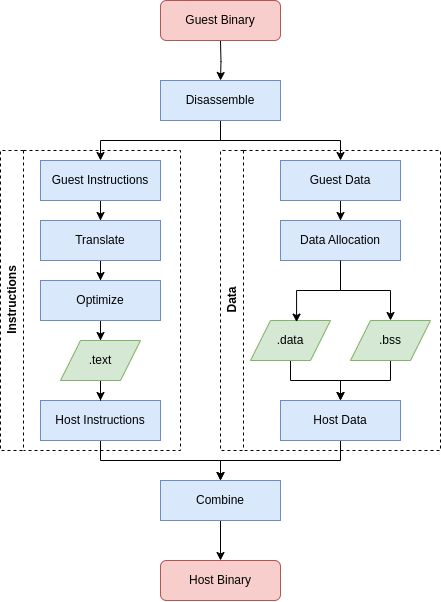
\includegraphics[width=0.6\linewidth]{figures/sta_bin_trans}
    \caption{Static Binary Translation}
    \label{fig:static_binary_translation}
\end{figure}

\subsection{Dynamic Binary Translation}
Dynamic translation is a subset of binary translation.
It involves translating binary code at runtime as the program executes.
Dynamic translation offers the advantage of adaptability, as it can optimize the translation based on the program's actual execution path, which may vary from run to run.

This method is especially useful in emulating complex software where it is impractical to predict all possible execution paths in advance.
However, it has some drawbacks regarding memory and performance.
When a dynamic translator is running, extra space is required for the program that is being translated.
It needs to allocate space for the disassembled program and the translated instructions.
This space may balloon very quickly at the start.
The other drawback is the performance penalty of translating instructions before executing them.
This drawback is also mostly evident in the starting phase when the cache is empty.
Overall, programs that use dynamic binary translation tend to take up a lot of resources at the start, which decreases after the initial starting phase.

As shown in figure \ref{fig:dynamic_binary_translation}, dynamic binary translators have a mechanism against the performance drawback.
They often incorporate a cache to store recently translated instructions, reducing the overhead of re-translating those instructions on subsequent executions. 
This caching mechanism is a key factor in mitigating the performance penalty associated with runtime translation, making dynamic translation an efficient and versatile approach for system emulation and virtualization environments.

\begin{figure}[ht]
    \centering
    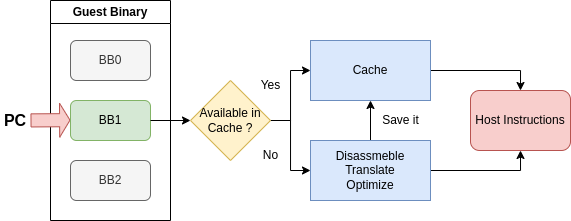
\includegraphics[width=0.8\linewidth]{figures/dyn_bin_trans}
    \caption{Dynamic Binary Translation}
    \label{fig:dynamic_binary_translation}
\end{figure}

\section{Basic Blocks}
In computer science, basic blocks are code sequences with a single entry point and no branches except at the exit.
In other words, basic blocks are chunks of code that will always run the same way and exit at the same point.
There is no branching in the middle, and the order of executed instructions are always the same.
This simplicity makes basic blocks easy to analyze.
Therefore, they are often used in compilers, optimizers, disassemblers, and reverse engineering tools.

\section{Emulators}

Computer emulators are software designed to mimic the ISA of a computer on another computer.
This allows software designed for the guest system to operate on the host system. 
In this section, we will go into detail about our primary targets.
Then, we will briefly explain the expected output of these emulators, which we use for analysis.

\subsection{QEMU}
\ac{QEMU} is a well-known free and open-source emulator and a virtualizer. 
At its core, \ac{QEMU} employs dynamic binary translation, which lets the host machine run programs belonging to a different architecture.
Enabling this is the \ac{TCG}, an integral part of \ac{QEMU} that dynamically generates native code for the host CPU.
As shown in figure \ref{fig:qemu_tcg} the \ac{TCG} is used to translate a guest \ac{ISA} into the host's architecture.

\begin{figure}[ht]
    \centering
    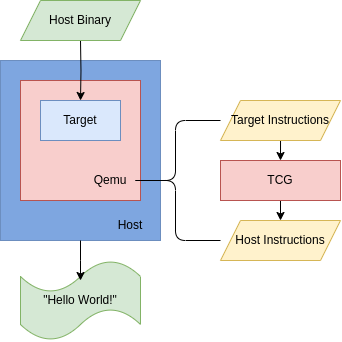
\includegraphics[width=0.7\linewidth]{figures/qemu_TCG2}
    \caption[QEMU translation process]{\ac{QEMU} translation process with \ac{TCG}}
    \label{fig:qemu_tcg}
\end{figure}

\subsubsection{TCG}
\ac{TCG} \cite{qemu_tcg}, which began as a generic backend for a C compiler, was later improved upon to be both portable and efficient, allowing \ac{QEMU} to quickly translate the guest instructions into a form that can be directly executed by the host machine, thereby improving the speed and efficiency of the emulation process.
This combination of dynamic binary translation and the flexibility of \ac{TCG} enables \ac{QEMU} to provide a high-performance and versatile solution for system emulation.
Thanks to the flexibility of the \ac{TCG}, many different architectures are supported by \ac{QEMU}.

These include \cite{qemu_arch}:
\begin{itemize}
    \item Arm
    \item MIPS (little endian)
    \item PPC
    \item RISC-V
    \item s390x
    \item SPARC
    \item x86
\end{itemize}

\subsection{Arancini}
Arancini is a project from the Systems Research Group at the \ac{TUM}.
It builds on the knowledge gained from two earlier projects: Lasagna \cite{rocha2022lasagne}, which translates any x86 program statically to an Arm \ac{ISA}, and Risotto \cite{gouicem2022risotto}, which emulates x86 program dynamically on an Arm machine.
Like these previous projects, Arancini focuses on making x86 programs work on Arm and adds support for RISC-V systems.
It achieves this by combining LLVM, a well-known toolkit for building compilers, with its own custom translation technology.

\subsection{Emulator Logs}
An emulator log is a detailed record of an emulator's operation.
It generally captures a wide range of information about the emulator's activities.
For our reproducer to function correctly, we must capture specific values after every instruction or basic block.
These values include register values and all reads and writes in order.
Generally, emulator logs include more information, including the executed instructions, the translated code, and more.
However, the aforementioned values are enough to know the exact state of the binary before executing the next step.

\section{Execution Methods}
\subsection{Concrete Execution}
Concrete execution refers to the traditional method of running programs, in which the program operates on actual, specific input values to produce outputs.
In this execution model, the program's instructions are carried out step by step, with each operation performed using concrete data values provided at runtime or predefined in the program. 
This straightforward method mirrors how programs are executed in real-world scenarios, making it intuitive and easy to understand. 

Concrete execution is particularly useful for debugging.
It allows developers to trace the exact sequence of steps a program takes with a given set of inputs, observing the program's behavior and output directly.
However, its reliance on specific inputs means that concrete execution can only explore one path through the program at a time, limiting its ability to uncover issues that may arise with different inputs or in untested execution paths.

\subsection{Symbolic Execution}
Symbolic execution, on the other hand, abstracts away from concrete input values, instead treating inputs as symbolic variables that can represent multiple possible values simultaneously. 
This approach allows the program to be executed in a way that explores multiple execution paths in a single run by considering all the possible values that the symbolic variables might take. 
Symbolic execution builds a mathematical model of the program's execution paths, using symbolic expressions to represent the outcome of computations and decisions based on the symbolic inputs. 
Figure \ref{fig:sym_tree} shows that every possible branching instruction adds a new path.
\begin{figure}[ht]
    \centering
    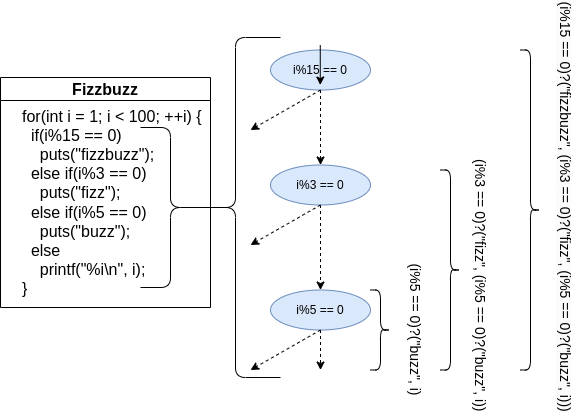
\includegraphics[width=0.8\linewidth]{figures/sym_trans}
    \caption[Branching in symbolic execution]{An example of a branching code in a tree}
    \label{fig:sym_tree}
\end{figure}

This model can then be analyzed to identify potential bugs, security vulnerabilities, or performance issues across a wide range of input conditions without having to enumerate and test each one individually. 
While powerful, symbolic execution is computationally intensive and can face challenges like path explosion, where the number of possible execution paths grows exponentially with the program's complexity.

\subsection{Concolic Execution} 
Concolic execution, a hybrid approach combining concrete and symbolic execution, aims to mitigate some of the limitations of both methods. 
In concolic execution, the program is run with specific concrete input values, like in concrete execution, but at the same time, it tracks symbolic constraints derived from the execution path taken. 
By analyzing these constraints, concolic execution tools can systematically generate new concrete inputs that will explore different paths through the program, thus eliminating state explosion in many cases.
% , combining the depth of symbolic analysis with the actual values from concrete execution.

This approach allows for more efficient exploration of the program's execution space, making it possible to uncover subtle bugs or vulnerabilities that might not be evident through conventional testing. 
Concolic execution has proven particularly useful in software testing and verification, providing a balance between the thoroughness of symbolic execution and the directness of concrete execution.

\section{Verifier}
In this section, we will explore the tools used to build the verifier step by step.

\subsection{Theorem Provers}
Theorem provers are computer programs that assist in proving mathematical theorems through formal methods.
The core idea behind theorem proving is to represent mathematical statements and proofs as formal structures that a computer can manipulate.
Theorem provers can then be used to check the validity of these proofs or even to automatically generate proofs for certain propositions within a given set of axioms and rules of inference.

\subsection{Miasm}
Miasm \cite{desclaux2012miasm} is a framework primarily designed for reverse engineering and binary analysis.
It features tools such as a disassembler and a symbolic execution engine.
The framework operates by taking advantage of the features of the symbolic execution engine, where binary code is interpreted in terms of symbolic expressions rather than concrete values.

This symbolic approach allows the theorem prover to evaluate the logical and mathematical properties of the code, solving constraints and proving or disproving theorems about the code's behavior under various conditions.
It also paints a clear picture of the transitions of the register and memory states between instructions and basic blocks.
The produced symbolic expressions are invaluable when comparing different states as they can pinpoint the expected and actual changes.

\subsection{Focaccia}
Focaccia is a specialized verifier program designed to assess the accuracy of emulators.
It uses concolic execution to collect data from a binary and compare it with an emulator's log.
At its core, Focaccia works by comparing two data sets.
The first data set comprises the memory and register values obtained during a test run on actual hardware, which serves as the benchmark or oracle for expected outcomes. 
The second data set involves a detailed log produced by the emulator during its operation, which records various actions, including register modifications, memory writes, and the current position of the \ac{PC}.
These logs are integral to the verification process as they provide a sequential record of the emulator's behavior, which lets Focaccia find the cutoff point where it starts to behave differently.

The verifier uses the Miasm \cite{desclaux2012miasm} reverse engineering framework for breaking down the original binary code into symbolic expressions for each operational step, transforming the instructions into a more abstract and analyzable form.
These symbolic expressions represent the ideal state changes that should occur step by step according to the software's design.
After collecting these symbolic expressions, they are compared with the state changes recorded in the emulator's log.

This comparison is the verifier's focal point, as it highlights any discrepancies between the expected behavior (as defined by the symbolic expressions) and the actual behavior observed in the emulator.
Discrepancies signal potential bugs in the emulator, indicating that the emulator's reproduction of hardware behavior is not entirely accurate.
